\documentclass[tikz,border=12pt]{standalone}
\usepackage[T1]{fontenc}
\usepackage{mathpazo}
\usepackage{amsmath,amssymb}
\usetikzlibrary{arrows.meta, positioning, calc}

\definecolor{stblue}{HTML}{7B97AD}
\definecolor{rwgold}{HTML}{B8995E}
\definecolor{sage}{HTML}{7A9A7E}
\definecolor{dkbrown}{HTML}{3D3530}
\definecolor{wmgray}{HTML}{7B7067}
\definecolor{cream}{HTML}{F9F6F0}
\definecolor{border}{HTML}{D4C9B8}
\definecolor{terracotta}{HTML}{C47A6A}

\begin{document}
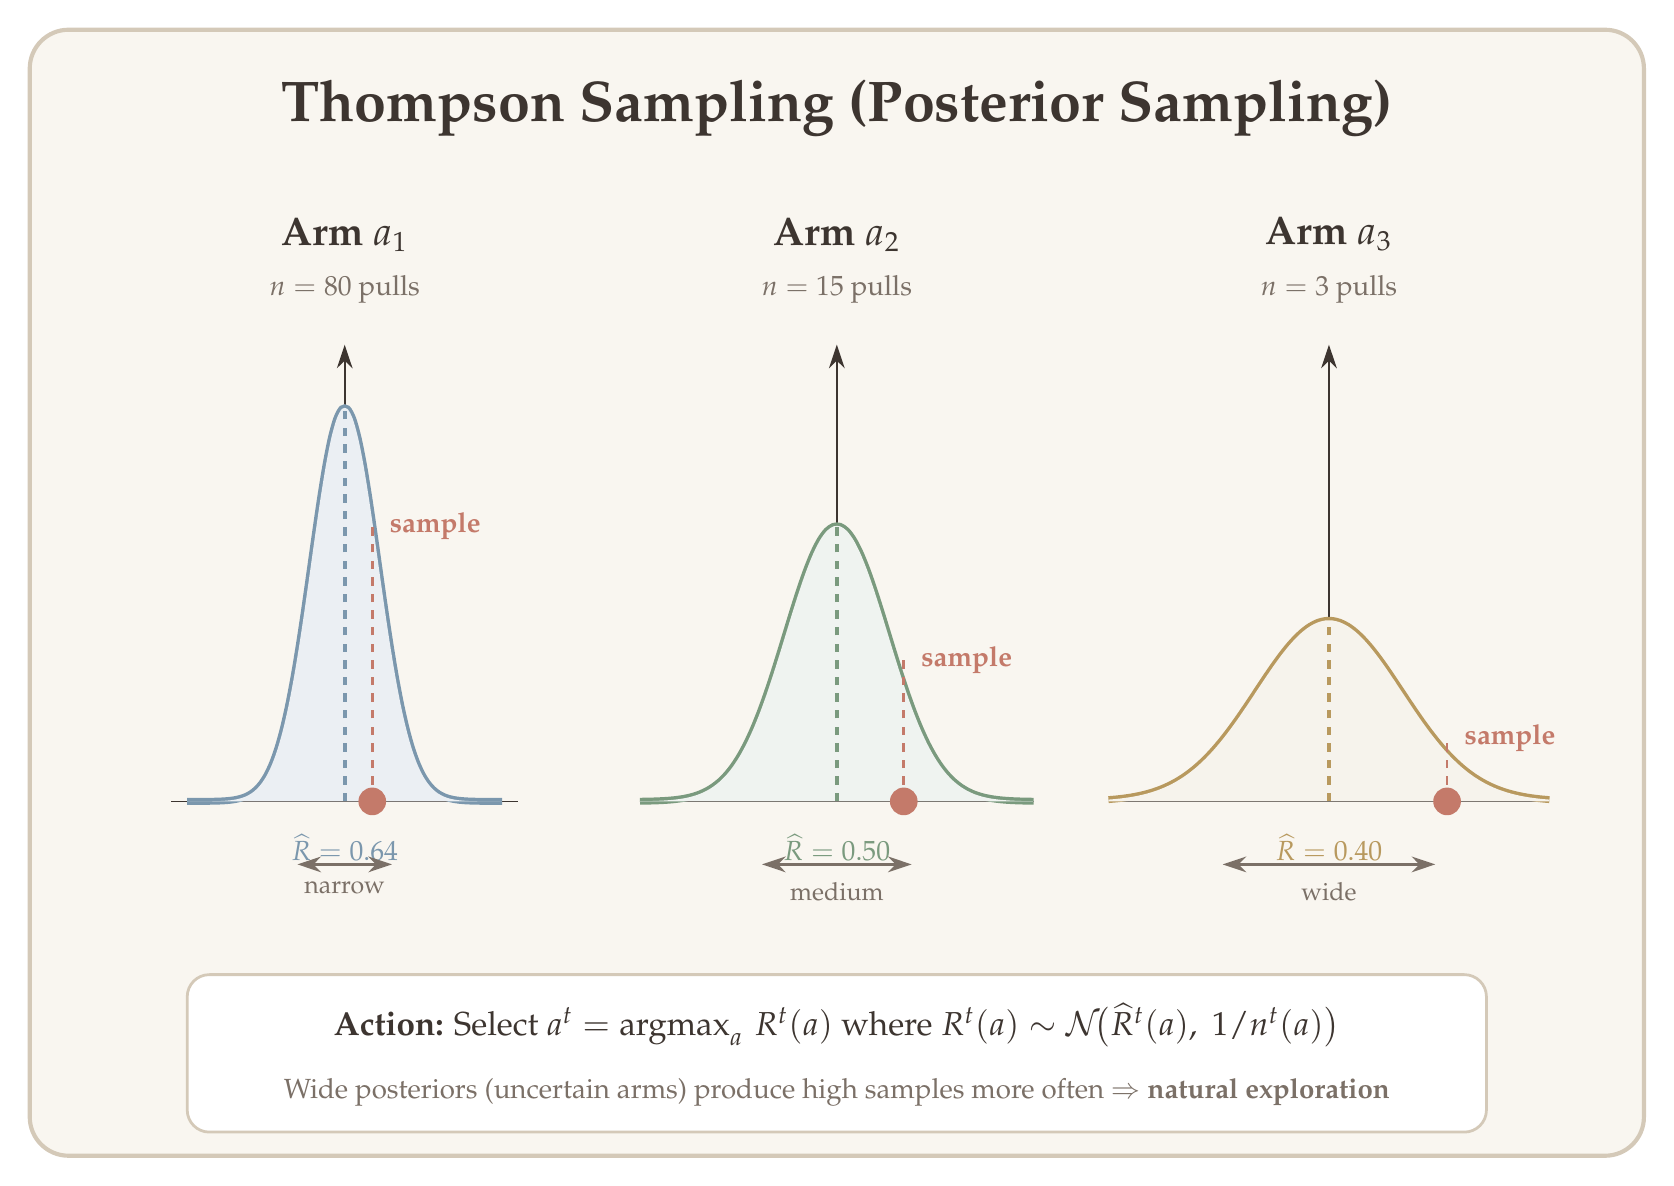
\begin{tikzpicture}[
  >={Stealth[length=3mm, width=2mm]},
]

% Background
\fill[cream, rounded corners=14pt] (-1.5,-4.5) rectangle (19,9.8);
\draw[border, rounded corners=14pt, line width=1.5pt] (-1.5,-4.5) rectangle (19,9.8);

% Title
\node[font=\huge\bfseries, text=dkbrown] at (8.75,8.8)
  {Thompson Sampling (Posterior Sampling)};

% =============================================
% Three arms with posterior distributions
% =============================================

% Gaussian curve helper: we draw sampled curves manually
% Arm 1: well-explored, narrow posterior, mean=0.64
\begin{scope}[shift={(2.5,0)}]
  \node[font=\Large\bfseries, text=dkbrown] at (0,7.2) {Arm $a_1$};
  \node[font=\normalsize, text=wmgray] at (0,6.5) {$n = 80$ pulls};

  % Posterior distribution (narrow Gaussian)
  \draw[dkbrown, line width=0.6pt] (-2.2,0) -- (2.2,0); % baseline
  \draw[dkbrown, line width=0.6pt, ->] (0,0) -- (0,5.8);

  % Posterior curve (narrow)
  \draw[stblue, line width=2.5pt, smooth] plot[domain=-2:2, samples=60]
    ({\x}, {5.0*exp(-(\x)^2/(2*0.18))});
  \fill[stblue!15, smooth] plot[domain=-2:2, samples=60]
    ({\x}, {5.0*exp(-(\x)^2/(2*0.18))}) -- (2,0) -- (-2,0) -- cycle;

  % True mean line
  \draw[stblue, line width=1.5pt, dashed] (0,0) -- (0,5.0);
  \node[font=\normalsize, text=stblue, below] at (0,-0.3) {$\widehat{R} = 0.64$};

  % Sample drawn (star)
  \fill[terracotta] (0.35, 0) circle (5pt);
  \draw[terracotta, line width=1pt, dashed] (0.35, 0) -- (0.35, 3.5);
  \node[font=\normalsize\bfseries, text=terracotta, right] at (0.45, 3.5) {sample};

  % Variance annotation
  \draw[wmgray, line width=0.8pt, <->] (-0.6, -0.8) -- (0.6, -0.8);
  \node[font=\small, text=wmgray, below] at (0,-0.9) {narrow};
\end{scope}

% Arm 2: moderately explored, medium posterior, mean=0.50
\begin{scope}[shift={(8.75,0)}]
  \node[font=\Large\bfseries, text=dkbrown] at (0,7.2) {Arm $a_2$};
  \node[font=\normalsize, text=wmgray] at (0,6.5) {$n = 15$ pulls};

  \draw[dkbrown, line width=0.6pt] (-2.5,0) -- (2.5,0);
  \draw[dkbrown, line width=0.6pt, ->] (0,0) -- (0,5.8);

  % Posterior curve (medium width)
  \draw[sage, line width=2.5pt, smooth] plot[domain=-2.5:2.5, samples=60]
    ({\x}, {3.5*exp(-(\x)^2/(2*0.42))});
  \fill[sage!12, smooth] plot[domain=-2.5:2.5, samples=60]
    ({\x}, {3.5*exp(-(\x)^2/(2*0.42))}) -- (2.5,0) -- (-2.5,0) -- cycle;

  \draw[sage, line width=1.5pt, dashed] (0,0) -- (0,3.5);
  \node[font=\normalsize, text=sage, below] at (0,-0.3) {$\widehat{R} = 0.50$};

  % Sample drawn (star) -- lucky high sample
  \fill[terracotta] (0.85, 0) circle (5pt);
  \draw[terracotta, line width=1pt, dashed] (0.85, 0) -- (0.85, 1.8);
  \node[font=\normalsize\bfseries, text=terracotta, right] at (0.95, 1.8) {sample};

  \draw[wmgray, line width=0.8pt, <->] (-0.95, -0.8) -- (0.95, -0.8);
  \node[font=\small, text=wmgray, below] at (0,-0.9) {medium};
\end{scope}

% Arm 3: poorly explored, wide posterior, mean=0.40
\begin{scope}[shift={(15,0)}]
  \node[font=\Large\bfseries, text=dkbrown] at (0,7.2) {Arm $a_3$};
  \node[font=\normalsize, text=wmgray] at (0,6.5) {$n = 3$ pulls};

  \draw[dkbrown, line width=0.6pt] (-2.8,0) -- (2.8,0);
  \draw[dkbrown, line width=0.6pt, ->] (0,0) -- (0,5.8);

  % Posterior curve (wide)
  \draw[rwgold, line width=2.5pt, smooth] plot[domain=-2.8:2.8, samples=60]
    ({\x}, {2.3*exp(-(\x)^2/(2*0.85))});
  \fill[rwgold!12, smooth] plot[domain=-2.8:2.8, samples=60]
    ({\x}, {2.3*exp(-(\x)^2/(2*0.85))}) -- (2.8,0) -- (-2.8,0) -- cycle;

  \draw[rwgold, line width=1.5pt, dashed] (0,0) -- (0,2.3);
  \node[font=\normalsize, text=rwgold, below] at (0,-0.3) {$\widehat{R} = 0.40$};

  % Sample drawn -- very high due to wide posterior
  \fill[terracotta] (1.5, 0) circle (5pt);
  \draw[terracotta, line width=1pt, dashed] (1.5, 0) -- (1.5, 0.8);
  \node[font=\normalsize\bfseries, text=terracotta, right] at (1.6, 0.8) {sample};

  \draw[wmgray, line width=0.8pt, <->] (-1.35, -0.8) -- (1.35, -0.8);
  \node[font=\small, text=wmgray, below] at (0,-0.9) {wide};
\end{scope}

% =============================================
% Bottom: Decision annotation
% =============================================
\fill[white, rounded corners=8pt] (0.5,-2.2) rectangle (17,-4.2);
\draw[border, rounded corners=8pt, line width=1pt] (0.5,-2.2) rectangle (17,-4.2);

\node[font=\large, text=dkbrown, align=left] at (8.75,-2.85)
  {\textbf{Action:} Select $a^t = \operatorname{argmax}_a\, R^t(a)$ where $R^t(a) \sim \mathcal{N}\!\bigl(\widehat{R}^t(a),\; 1/n^t(a)\bigr)$};
\node[font=\normalsize, text=wmgray, align=center] at (8.75,-3.7)
  {Wide posteriors (uncertain arms) produce high samples more often $\Rightarrow$ \textbf{natural exploration}};

\end{tikzpicture}
\end{document}
